\documentclass[12]{beamer}
\usepackage{multicol}
\usepackage{enumitem}
\usepackage[obeyspaces]{url}
\usepackage{listings}
\lstnewenvironment{python}{\lstset{language=python}}{}
\lstnewenvironment{java}{\lstset{style=customjava,language=java}}{}

\lstdefinestyle{customjava}{
  belowcaptionskip=1\baselineskip,
  breaklines=true,
  language=java,
  showstringspaces=false,
  basicstyle=\footnotesize\ttfamily,
  keywordstyle=\bfseries\color{green!40!black},
  commentstyle=\itshape\color{purple!40!black},
  identifierstyle=\color{blue},
  stringstyle=\color{orange},
}

\usetheme[progressbar=frametitle]{metropolis}
\setbeamertemplate{frame numbering}[fraction]
\usefonttheme{metropolis}
\usecolortheme{spruce}
\setbeamercolor{background canvas}{bg=white}

\definecolor{mygreen}{rgb}{125, 5, 25}
\usecolortheme[named=mygreen]{structure}



\title{Assignment Two}
\author{Brae \& Emily \& Tom}
%\institute{ajou university.}
\institute {CSSE2002: Programming in the Large}

\setbeamercovered{transparent=5}


\begin{document}
\metroset{block=fill}
\begin{frame}
\titlepage
\end{frame}

\begin{frame}[t]{Getting Started} \vspace{4pt}
% \begin{block}{What is a UML Diagram?}
% \vspace{0.5em}
% A \textbf{UML Diagram} is a diagram which represents the relationships
% between classes. It is used to show which instances of classes another
% class holds and inheritance relationships.
% \vspace{0.5em}
% \end{block}

\begin{enumerate}[label*=\arabic*.]
	\item Download \path{supplied.zip} and \path{doc.zip} from blackboard
	\item Load the extracted contents of \path{supplied.zip} into IntelliJ - refer to week two slides
\end{enumerate}

\only<2>{The supplied code \textbf{will not compile} when initially loaded. Some code needs to be written (by you) before it will compile. This is stated in the task sheet.}

\end{frame}

\begin{frame}[t]{Where To Start?} \vspace{4pt}

Start with classes that don't have dependencies (e.g. Pair) \\
\onslide<2->{ \textbf{MapIO is hard} } \onslide<3->{ (IO has not yet been covered) }\\
Start with classes top of the hierarchy (e.g. Thing)\\[50pt]
\onslide<4->{The order specified in the task sheet is a good starting point}

\end{frame}

\begin{frame}[t]{What Has Changed?} \vspace{4pt}
\begin{center}
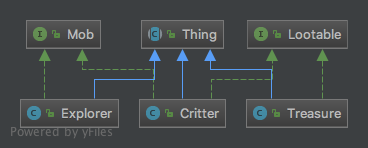
\includegraphics[scale=0.45]{old_classes}\\[20pt]
\only<2>{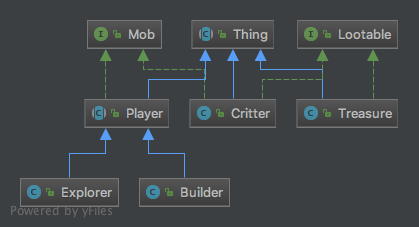
\includegraphics[scale=0.45]{new_classes}}
\end{center}
\end{frame}

\begin{frame}[t, fragile]{Joel's Solution} \vspace{4pt}

In Joel's solution he has used \texttt{Collections.unmodifiableList} and \texttt{Collections.unmodifiableMap} when returning a instance variables. Do I need to know this?

\only<2->{No. You were not expected to know these methods.}

\begin{onlyenv}<3->
\begin{java}
return Collections.unmodifiableList(this.contents);

return new ArrayList<Thing>(this.contents);

List<Thing> results = new ArrayList<Thing>();
for (Thing thing : this.contents) {
	results.add(thing);
}
return results;
\end{java}
\end{onlyenv}

\end{frame}

\begin{frame}[t, fragile]{Exceptions} \vspace{4pt}

Exceptions do not need to be complicated.

\begin{java}
public class CrawlException extends Exception {}

public class NullRoomException extends CrawlException {}
\end{java}

There is no need to add a constructor or any extra methods to exceptions.

\end{frame}

\begin{frame}[t, fragile]{Common Mistakes - Abstract Thing} \vspace{4pt}
The JavaDocs specified that the \texttt{Thing} class was an abstract class.

\begin{java}
public class Thing {
	...
}

public abstract class Thing {
	...
}
\end{java}
\end{frame}

\begin{frame}[t, fragile]{Common Mistakes - Code Duplication} \vspace{4pt}
Code duplication for replacing strings.

\begin{onlyenv}<2>
\textbf{Don't do this}
\begin{java}
public Thing(String shortDescription, String longDescription) {
    this.shortDescription = shortDescription.replace('\n', '*').replace(';', '*').replace('\r', '*');
    this.longDescription = longDescription.replace('\n', '*').replace(';', '*').replace('\r', '*');
}

protected void setShort(String shortDescription) {
    this.shortDescription = shortDescription.replace('\n', '*').replace(';', '*').replace('\r', '*');
}
\end{java}
\end{onlyenv}

\begin{onlyenv}<3>
Abstract away repeated code
\begin{java}
public Thing(String shortDescription, String longDescription) {
    this.shortDescription = replaceDescription(shortDescription);
    this.longDescription = replaceDescription(shortDescription);
}

private String replaceDescrition(String description) {
    return description.replace('\n', '*')
            .replace(';', '*')
            .replace('\r', '*');
}
\end{java}
\end{onlyenv}

\end{frame}

\begin{frame}[t, fragile]{Common Mistakes - String Comparison} \vspace{4pt}

Strings need to be compared using the .equals method not the comparison operator.

\begin{java}
String first = "hello";
String second = "hello";

if (first == second) {} // wrong
if (first.equals(second)) {} // right
\end{java}

\end{frame}

\begin{frame}[t, fragile]{Common Mistakes - Style} \vspace{4pt}
Horizontal space is required on both sides of any binary or ternary operator.

Separate any reserved word, such as if, for or catch, from an open parenthesis (() that follows it on that line.

\begin{java}
if (x) {} // right
if(x){} //wrong
if (x){} //wrong
if(x) {} //wrong
\end{java}

\end{frame}

\begin{frame}[t, fragile]{Common Mistakes - Style} \vspace{4pt}

\begin{block}{Name Case}
\textbf{Variable names} should be in camelCase\\
\textbf{Class names} should be in PascalCase\\
\textbf{Constants} should be in \verb|SCREAMING_SNAKE_CASE|\\
\textbf{Method names} should be in camelCase\\[10pt]
\end{block}

\begin{onlyenv}<2->
\begin{java}
public class MyClassName {
	private static final int MAX_SCORE = 1000;
	private int bestScore = 0;

	public int getBestScore() {
		int myScore = 1;
		return myScore;
	}
}
\end{java}
\end{onlyenv}
\end{frame}

\begin{frame}[t, fragile]{Common Mistakes - Style} \vspace{4pt}

More on style in your tutorials...

\end{frame}

\end{document}
